\documentclass[12pt,letterpaper]{article}
\usepackage{fullpage}
\usepackage[top=2cm, bottom=4.5cm, left=2.5cm, right=2.5cm]{geometry}
\usepackage{amsmath,amsthm,amsfonts,amssymb,amscd}
\usepackage{lastpage}
\usepackage{enumerate}
\usepackage{fancyhdr}
\usepackage{mathrsfs}
\usepackage{xcolor}
\usepackage{graphicx}
\usepackage{hyperref}
\usepackage{sectsty}
\usepackage{enumitem}
\usepackage{siunitx}
\usepackage{stackengine}
\usepackage{subcaption}
\usepackage{scalerel}
\usepackage{pdfpages}


\sectionfont{\fontsize{14.4}{17}\selectfont}
\subsectionfont{\fontsize{10}{12}\selectfont}

\hypersetup{%
  colorlinks=true,
  linkcolor=blue,
  linkbordercolor={0 0 1}
}

\setlength{\parindent}{0.0in}
\setlength{\parskip}{0.05in}

% Edit these as appropriate
\newcommand\course{CMPE 670}
\newcommand\hwnumber{2}
\newcommand\NetIDa{Andrei Tumbar}

\pagestyle{fancyplain}
\headheight 35pt
\lhead{\NetIDa}
\chead{\textbf{\Large Homework \hwnumber}}
\rhead{\course \\ \today}
\lfoot{}
\cfoot{}
\rfoot{\small\thepage}
\headsep 1.5em


% Long division commands
\newcommand\showdiv[1]{\overline{\smash{\hstretch{.5}{)}\mkern-3.2mu\hstretch{.5}{)}}#1}}
\let\ph\phantom

\begin{document}

\section*{Question 1}

\begin{verbatim}
           11100000011
     -----------------
1101 ) 101101100101000
      -01101
      ------
        10011
       -01101
       ------
          1101
         -1101
         -----
                10100
               -01101
               ------
                  1110
                 -1101
                 -----
                     1

CRC: 001
Msg: 101101100101001
\end{verbatim}

\section*{Question 2}

\subsection*{a) See below for Bellman-Ford and Dijkstra rounting tables}
It took four iterations (including the initialization) to complete the Bellman-Ford
algorithm over all of the nodes. The order in which the edges are evaluated will not
have an effect of the final output of the algorithm though it may or may not settle
some nodes in earlier iterations.

\subsection*{c)}
The Bellman Ford algorithm will send fewer messages but it must synchronize its
messages over all of the nodes. This operation may cause considerable slowdown.
Dijkstra's algorithm will require more network bandwidth as each node will perform
its resolution of the entire network on its own. Put simpler, Bellman Ford will
require all the nodes to work together to build the routing table, whereas Dijkstra
will require each individual node to build the table on its own.

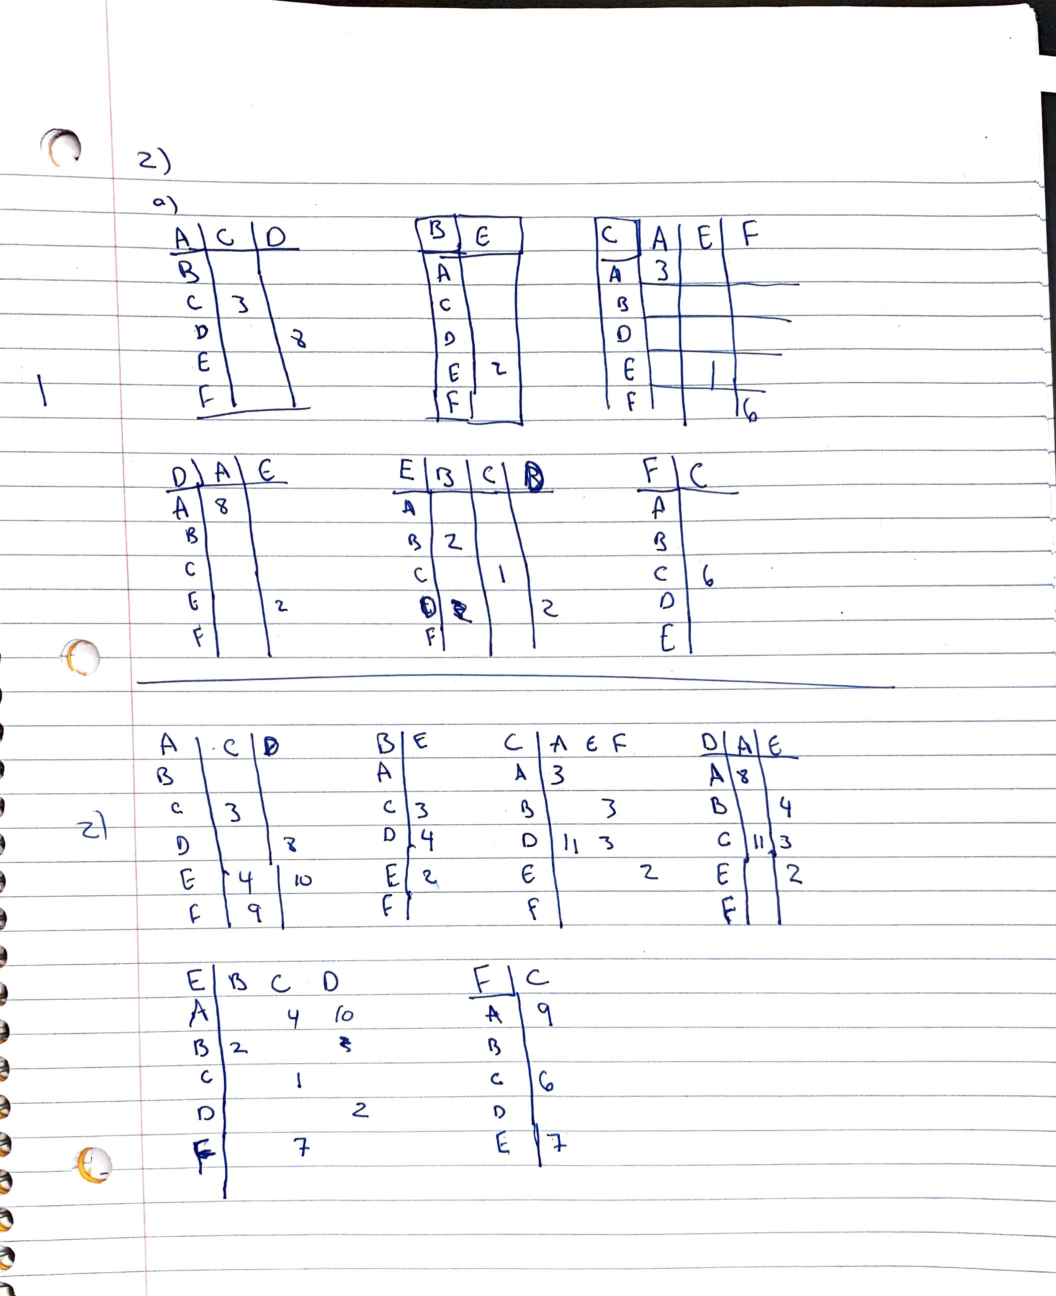
\includepdf[pages=-,pagecommand={},width=\textwidth]{670-part2.pdf}

\section*{Question 3}
After the 3rd collision, the algorithm will chose between $2^3$ different delay times.
Each of the 8 options have equal probability of being chosen as the distribution is
uniform. This means \SI{153.6}{\micro\s} will have a $0.125$ probablity of being
chosen.

\section*{Question 4}
There needs to be a minimum frame size so that the sender can detect collision if
there is one. If the frame size is too short then the collision would be detected
after the transmission has already been completed. This relates to acknoledgment
because if no collision is detected during transmission, the transmitter can
know if the transmission successfully reached the destination.

\section*{Question 5}
ALOHA is best when the carrier delay is large. This is because CSMA/CD will require a
minimum frame-size proportional to the carrier delay. Making the minimum frame size
too large will make the probality of collision extremely high and cause deadlock in
the network.\\

CSMA/CD should be chosen when the carrier delay is relatively low. This will allow
for reliable short transmitions across the network. Carrier delay should be below
the packet transmission delay to keep line mostly free of collisions.

\end{document}
